\chapter{Desenvolvimento de uma Rede Social de Colaborações e Aprendizagem}
\label{desen-noosferAVA}

Neste capítulo será apresentado o processo para a implementação das funcionalidades apresentadas na Secão \ref{historia-usuario}, mostrando os passos de desenvolvimento do \textit{plugin WorkAssignment} e Comunidade.UnB para o Noosfero, bem como os resultados obtidos. 

% ----------------------------------------------------------------
\section{O processo de desenvolvimento}

O desenvolvimento foi realizado no Laboratório de Produção, Pesquisa e Inovação em Software (LAPPIS) da FGA que é um ambiente para  alunos e professores trabalharem de forma colaborativa na produção de software. No laboratório são adotadas práticas ágeis onde vários de seus integrantes colaboram com o Noosfero.

A partir dos requisitos especificados e validadeos e levando em consideração as práticas ágeis utilizadas no LAPPIS foram realizadas \textit{sprints} com duração de quinze dias. Em cada \textit{sprint} foram desenvolvidas histórias de acordo com a pontuação e demanda de atividades na equipe do Portal, visto que o desenvolvimento foi realizado de maneira colaborativa.

\begin{figure}[h]
    \centering
    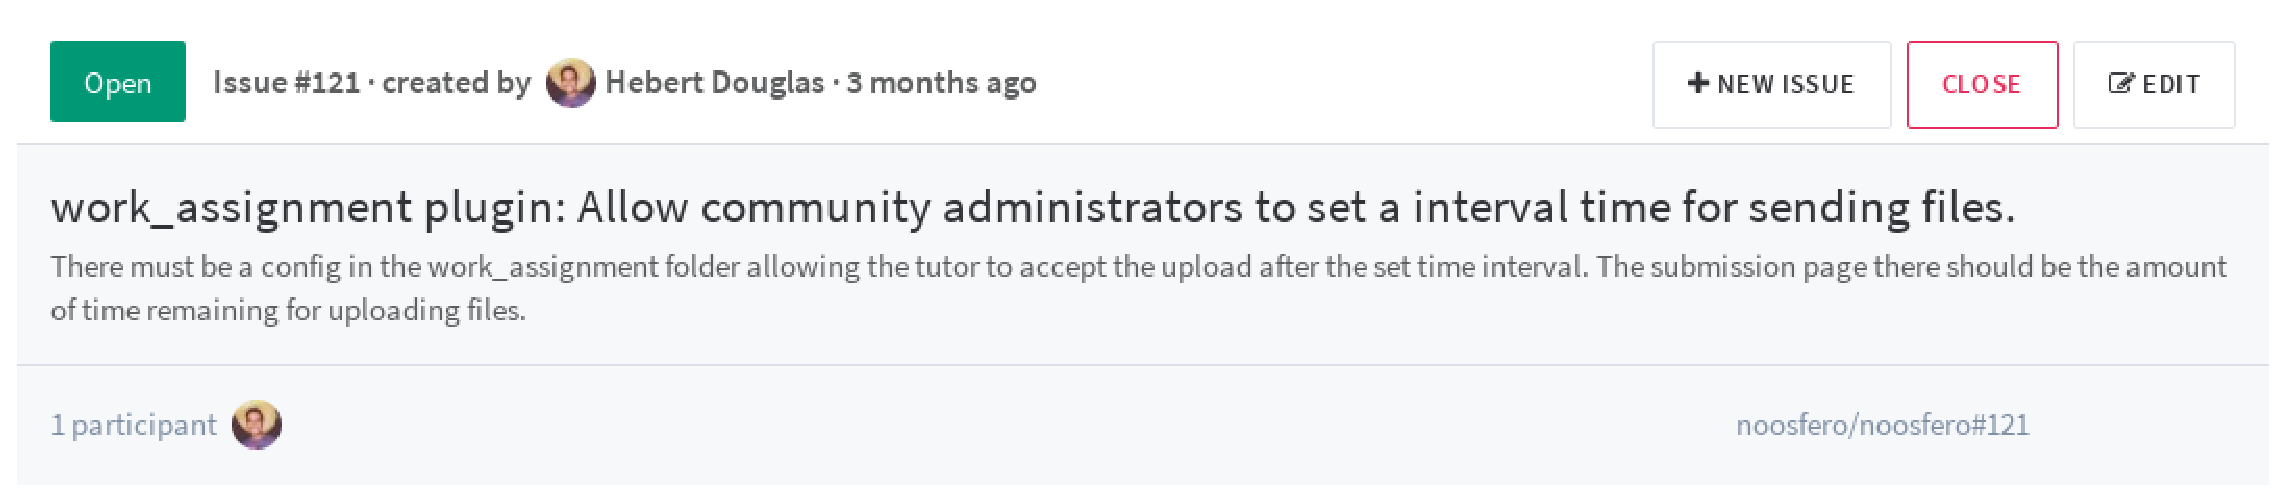
\includegraphics[keepaspectratio=true,scale=0.4]
      {figuras/issue121.eps}
    \caption{Issue 121: Gerenciamento de tempo para work\_assignment}
    \label{fig:issue-121}
\end{figure}

A primeira \textit{sprint} de desenvolvimento das histórias de usuário foi iniciada em julho com a equipe do Portal FGA. Seguindo as práticas de desenvolvimento da comunidade Noosfero, criou-se uma \textit{Issue} para evidenciar aos desenvolvedores o ínicio da implementação de uma nova funcionalidade. A \textit{Issue} criada foi a de número 121\footnote{Disponível em: \url{https://gitlab.com/noosfero/noosfero/issues/121}} que  é evidenciada na Figura \ref{fig:issue-121}.

Nessa sprint foi desenvolvida a história de usuário (\ref{us01}) ``Definir tempo restante'', que permite ao administrador definir e modificar um tempo limite para envio dos trabalhos no \textit{plugin work assignment}.

Na segunda sprint, foi desenvolvido o último cenário de uso da \ref{us01}, ``Permitir entrega de atividades após período''. Este cenário permite ao professor autorizar os alunos a enviarem suas atividades após o prazo definido. Além de implementar a história ``Visualizar tempo restante de atividades'' (\ref{us02}), que trata o modo de visualização do tempo restante para envio das atividades.

É importante ressaltar que na implementação das histórias \ref{us01} e \ref{us02} tem-se um exemplo prático de utilização dos \textit{hotspots} da arquitetura do Noosfero. No código \ref{cod:hotspot}, faz-se uso do \textit{hotspot} denominado como \textit{content\_remove\_upload}, utilizado para habilitar ou desabilitar a opção de upload de arquivos. Este código está contido no plugin e através dos métodos \textit{dispatch} é invocado pela classe responsável por gerenciar os \textit{plugins}.

\begin{lstlisting}[language=Ruby, caption={Código de implementação do \textit{hotspot}}, label=cod:hotspot]
  def content_remove_upload(content)
    if content.kind_of?(WorkAssignmentPlugin::WorkAssignment)
      !content.profile.members.include?(context.send(:user)) || (content.expired? && !content.ignore_time)
    end
  end
\end{lstlisting}

\begin{figure}[h]
    \centering
    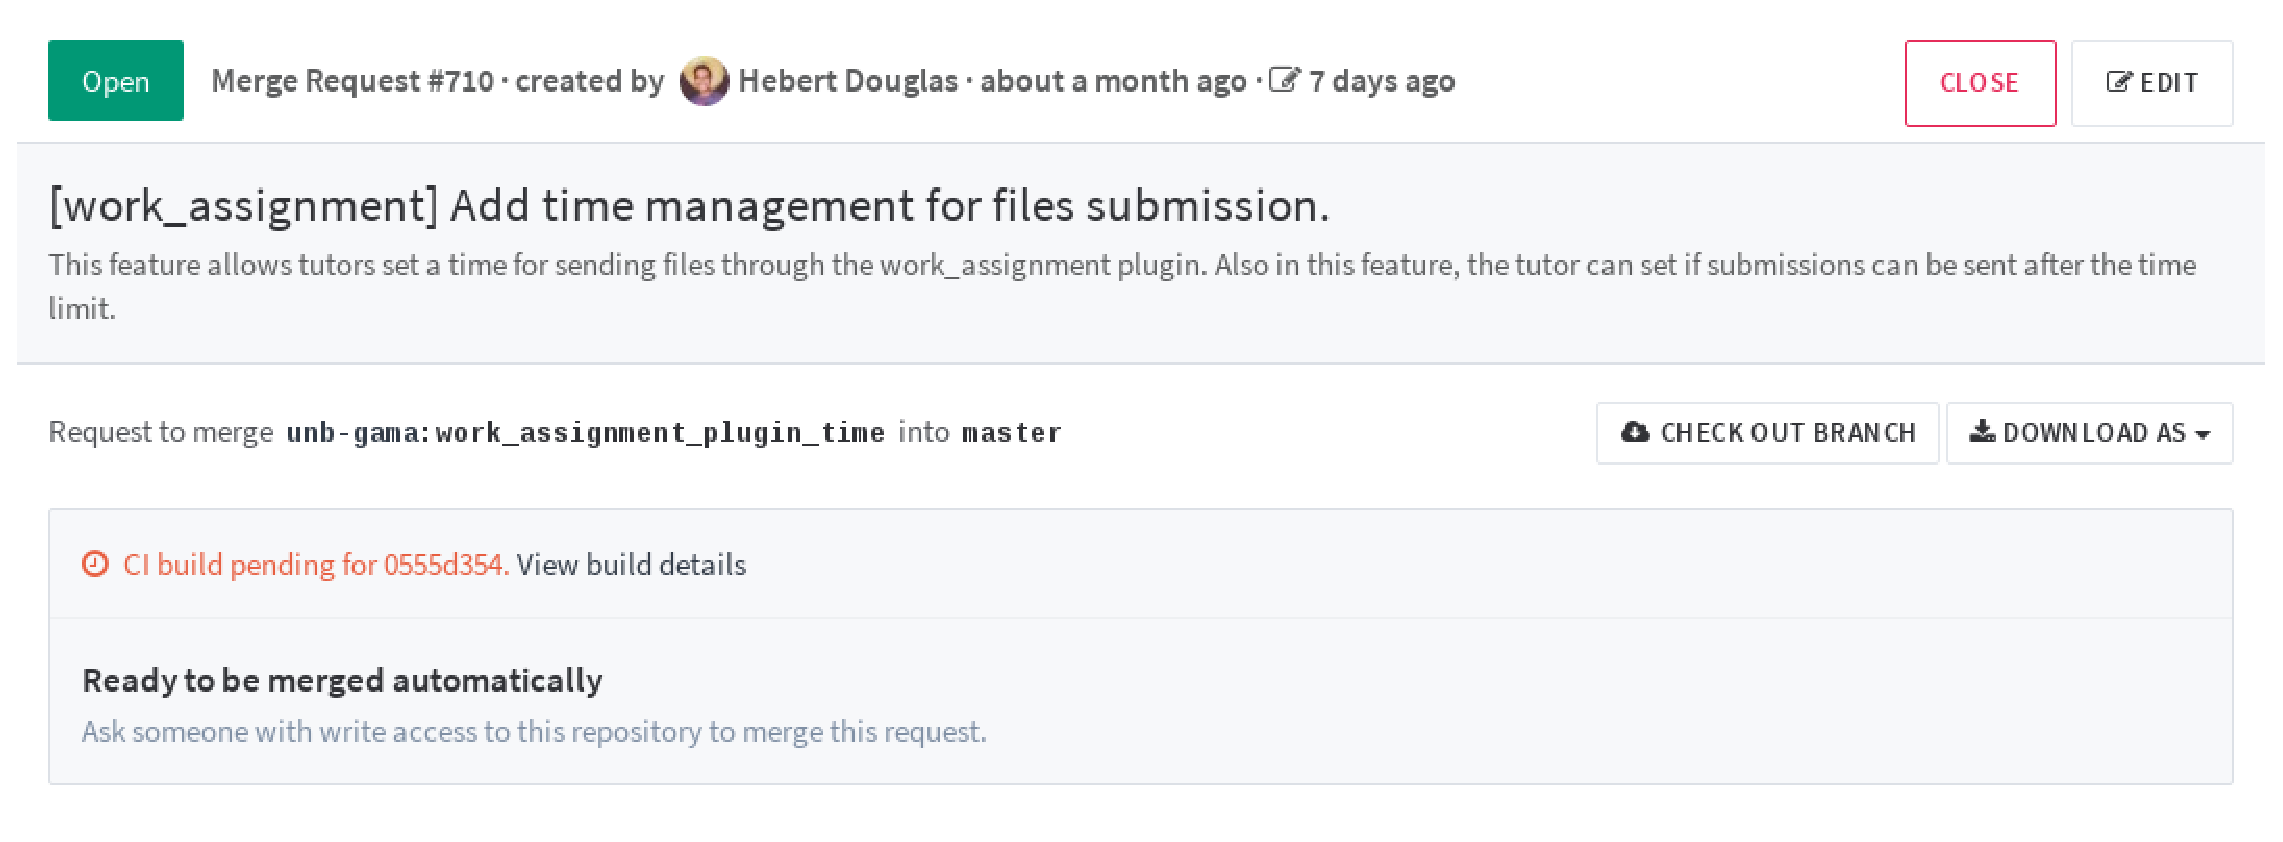
\includegraphics[keepaspectratio=true,scale=0.42]
      {figuras/merge-request710.eps}
    \caption{Merge Request: Gerenciamento de tempo para work\_assignment}
    \label{fig:merge-710}
\end{figure}

A implementação foi revisada por um dos integrantes do LAPPIS que sugeriu melhorias pontuais, resolvidas durante a revisão. Posteriormente foi realizado o \textit{Merge Request} para a integração do código à \textit{branch \textbf{master}} do Noosfero. Criou-se o Merge Request de número 710\footnote{Disponível em: \url{https://gitlab.com/noosfero/noosfero/merge_requests/710}} (Figura \ref{fig:merge-710}) que ficou em aberto para a revisão dos colaboradores oficiais da Comunidade. Após alguns dias o mesmo foi revisado pelos desenvolvedores do core do Noosfero, que aprovou a funcionalidade e indicou que será integrada ao Noosfero na versão 1\.4.

\begin{figure}[h]
    \centering
    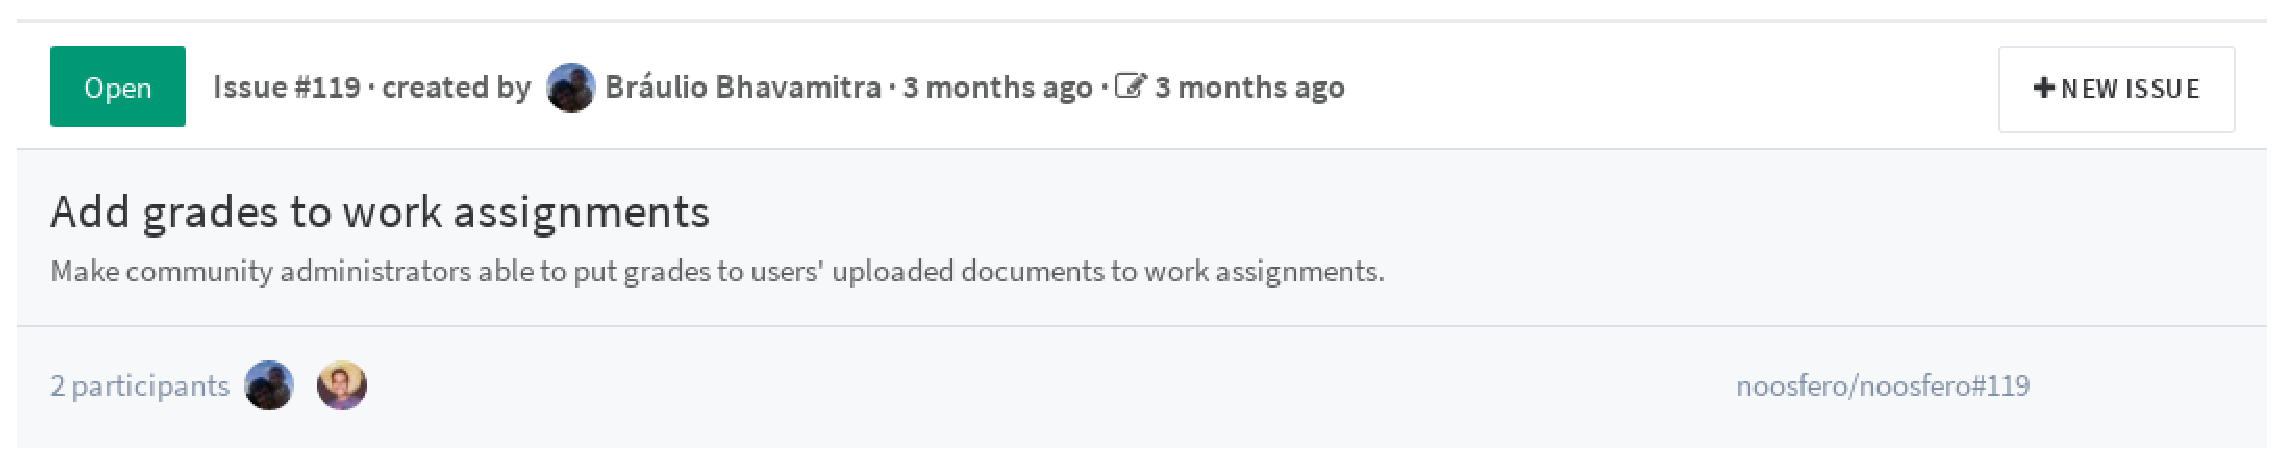
\includegraphics[keepaspectratio=true,scale=0.4]
      {figuras/issue119.eps}
    \caption{Issue 119: Adicionar notas ao \textit{plugin Work Assignment}}
    \label{fig:issue-119}
\end{figure}

A terceira \textit{sprint}, que engloba a história (\ref{us03}) ``Atribuir notas aos alunos''. No início da implementação verificou-se que esta funcionalidade já havia sido mapeada por integrante do Noosfero na \textit{Issue} 119 \footnote{Disponível em: \url{https://gitlab.com/noosfero/noosfero/issues/119}} (Figura \ref{fig:issue-119}), o que favoreceu o desenvolvimento, e evidenciou que o desenvolvimento na comunidade é feito de maneira colaborativa.

Também foram discutidas questões técnicas e arquiteturais relativas à implementação. As principais discussões giraram em torno das formas de realização da pontuação (por versões ou por pasta) e de atribuição da nota final do aluno. Ficou definido que todas as versões de arquivos enviados poderiam ser pontuados pelos administradores da comunidade e que em uma próxima \textit{sprint} seraim estabelecidos os critérios para definir a nota final do aluno.

Na quarta \textit{Sprint}, prosseguiu-se com o desenvolvimento da \ref{us03}, momento em que foi implementado o cenário de uso que proporciona ao administrador definir o critério para a nota final de cada atividade.  Além disso, foi implementada a história (\ref{us04}) ``Publicar notas aos alunos'', que permite ao administrador publicar ou omitir notas aos alunos. 

As funcionalidades desenvolvidas até então englobavam requisitos importantes de um AVA, conforme a Seção \ref{ava}, mas ainda não possibilitam visualização das notas pelo aluno.

Sendo assim na quinta \textit{sprint} foi implementada a história (\ref{us05}) ``Visualização das notas'', restrita à apresentação da tela de visualização das tarefas enviadas. Para que os membros da equipe realizassem uma avalição relativas ao \textit{design}.

Foi implementada a história (\ref{us06}) ``Professor gerencia notas'', que permite ao professor definir módulos que agrupem as atividades a serem enviadas. O objetivo principal dessa história é permitir ao administrador modularizar as atividades. O cenário ``Visualizar notas de todos ao alunos de um grupo de atividades'' não foi implementado, em vista do elevado número de requisições ao banco de dados e pequeno retorno ao usuário.

Como dívida técnica da quinta, na sexta \textit{sprint} foi implementado o cenário de uso ``Visualizar notas de todos os alunos de uma determinada atividade'' da \ref{us06}. A ideia principal é disponibilizar ao usuário, de maneira centralizada, a visualização de suas notas relativas a todas as atividades e módulos das comunidades nas quais está vinculado.

Na sétima \textit{sprint} foi implementada a história (\ref{us07}) ``Blocos de notas recentes'', que visa a criação de um bloco e exibe ao usuário as cinco notas recentes. Devido as sugestões de membros da comunidade houve uma evolução e padronização de telas do sistema.

Para oitava \textit{sprint} foi sugerida a criação de um bloco para visualização de todos os grupos e respectivas atividades. Esta funcionalidade está listada na \ref{us08} (``Bloco para visualização dos módulos'') e foi implementada em paralelo com os testes da história anterior.

\begin{figure}[h]
    \centering
    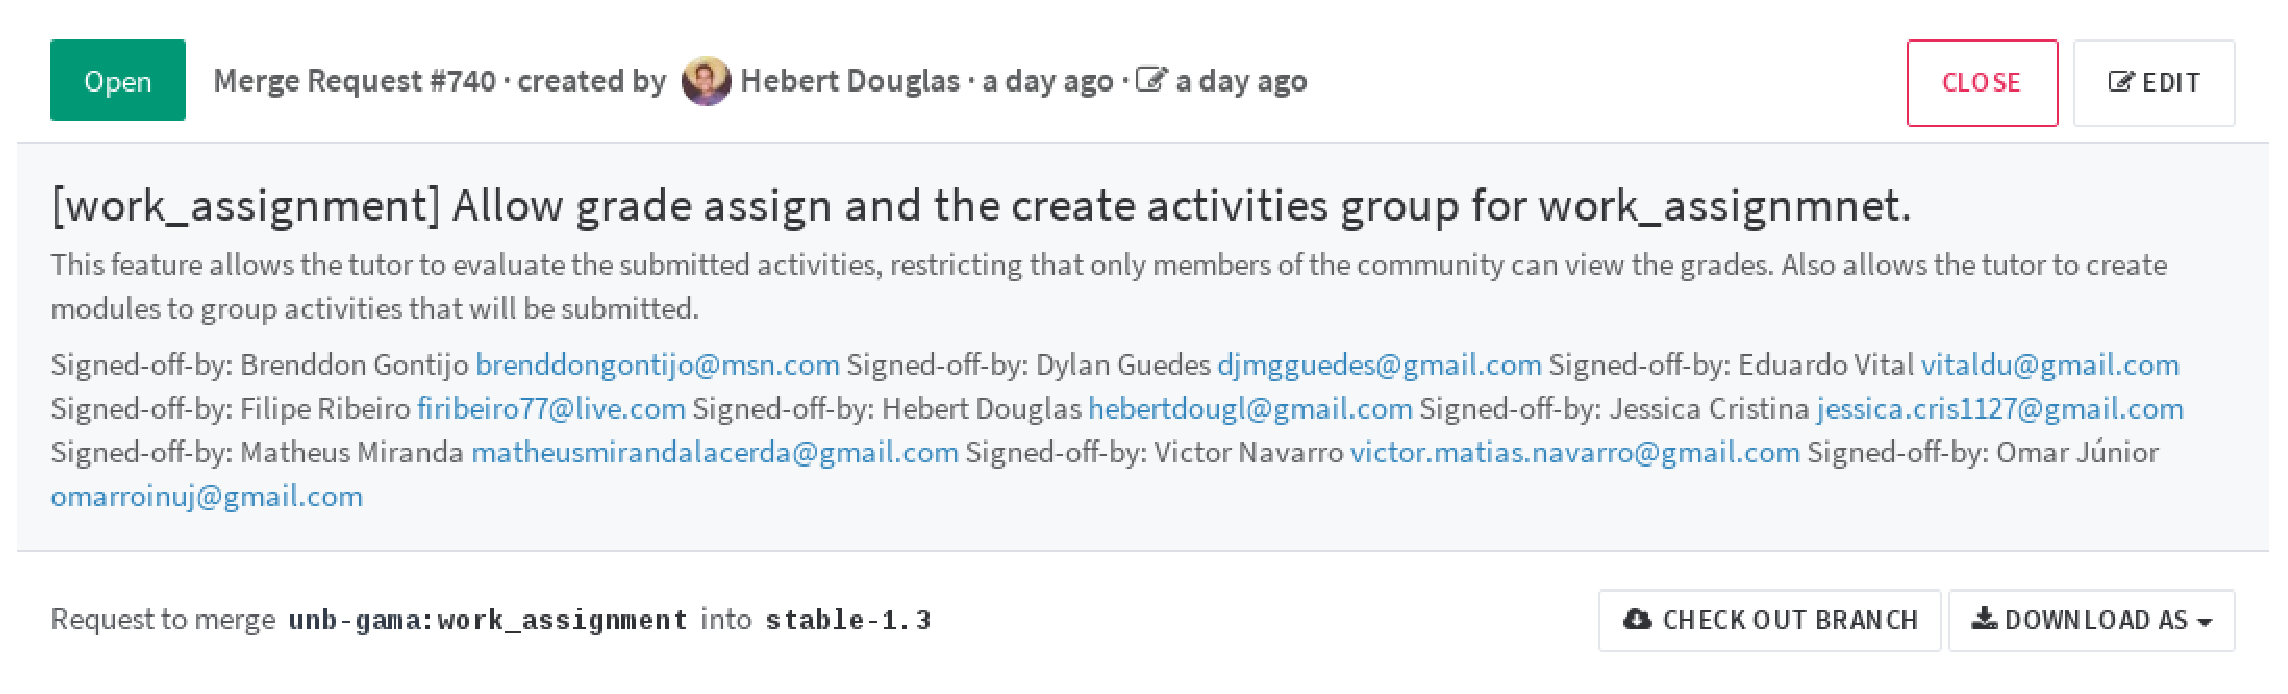
\includegraphics[keepaspectratio=true,scale=0.42]
      {figuras/merge-740.eps}
    \caption{Merge Request: Sistema de notas e módulos para work\_assignment}
    \label{fig:merge-740}
\end{figure}

Finalizada a execução dessas \textit{sprints}, foi realizado o \textit{Merge Request} para a integração do código à \textit{branch \textbf{master}} do Noosfero. Criou-se o Merge Request de número 740\footnote{Disponível em: \url{https://gitlab.com/noosfero/noosfero/merge_requests/740}} (Figura \ref{fig:merge-740}) que ficou em aberto para a revisão dos \textit{commiters} oficiais da Comunidade.

Na nona e última \textit{sprint} foi criado um ambiente de homologação para o Comunidade.UnB, com vistas a propiciar o teste das novas funcionalidades e a autenticação com o LDAP, relatados na \ref{us09}. Para validar o novo mecanismo de autenticação o CPD da FGA forneceu acesso a base de dados do seu servidor LDAP, apenas uma cópia de uma versão antiga a utilizada para o controle de acesso a rede \textit{wireless} do campus, e durante os testes no servidor de homologação a funcionalidade teve o comportamento esperado.

Nesse processo de desenvolvimento fica evidente a aplicação das práticas adotadas pela comunidade de software livre Noosfero. Foi executado o processo desde a criação de uma \textit{Issue}, passando por todo o processo de desenvolvimento adotando práticas ágeis, até o encerramento do ciclo com a criação do \textit{Merge request}. Vale lembrar que mesmo após a revisão e integração ao \textit{core} o código ainda se encontra em constante evolução.

% -------------------- Evolução do Work Assignment ----------------
\section{A evolução do \textit{plugin Work Assignment}}

Nesta seção serão apresentados os resultados correspondentes à evolução do \textit{plugin Work Assignment}, que até então possuía apenas a funcionalidade para permitir o envio de arquivos para o servidor em um determinado período de tempo.

O professor deve atribuir notas às atividades enviadas e acompanhar a situação de cada aluno. O aluno poderá visualizar todas as notas das atividades em cada disciplina, avaliando se o seu desempenho está satisfatório. Nesse contexto foram realizadas melhorias para propiciar tais funcionalidades.

As evoluções realizadas no \textit{plugin Work Assignment} permitem que o administrador de uma comunidade (professor), realize a modularização das atividades a serem entregues, propiciando-lhe a organização do curso e melhor visualização dos alunos.

Ao definir um módulo para seu curso, o professor informa a data de início e fim para o mesmo e, dessa maneira todas as atividades que farão parte desse módulo devem estar entre o período determinado.

\begin{figure}[h]
    \centering
    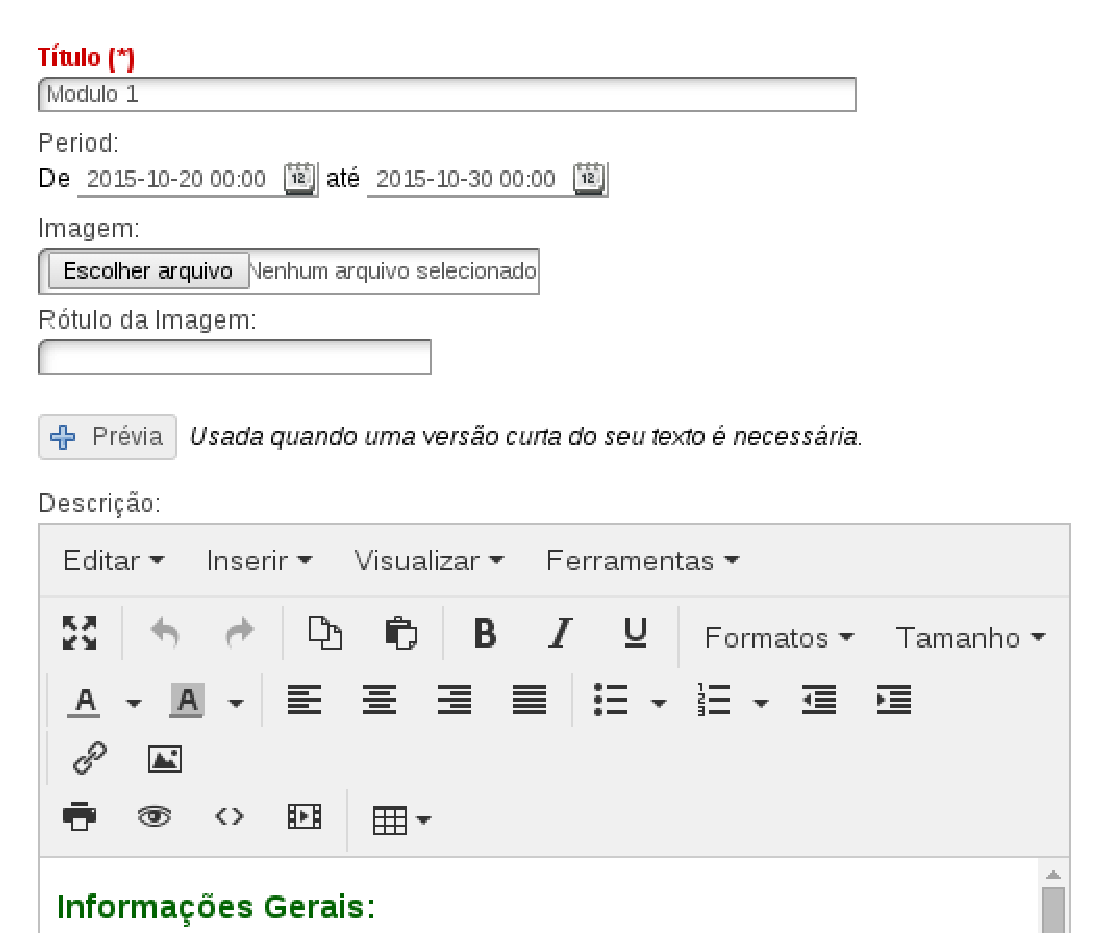
\includegraphics[keepaspectratio=true,scale=0.6]
      {figuras/work-assignment-group.eps}
    \caption{Tela para criação de grupos de trabalhos a serem enviados.}
    \label{fig:work-assignment-group}
\end{figure}

Para criar um módulo o administrador agora pode entrar no painel de controle da comunidade e adicionar um novo tipo de conteúdo denominado ``Grupo de Trabalhos a serem enviados''. Nesse conteúdo o usuário deve informar título, período, uma prévia do que será aquele módulo e sua descrição detalhada, conforme a Figura \ref{fig:work-assignment-group}.

\begin{figure}[h]
    \centering
    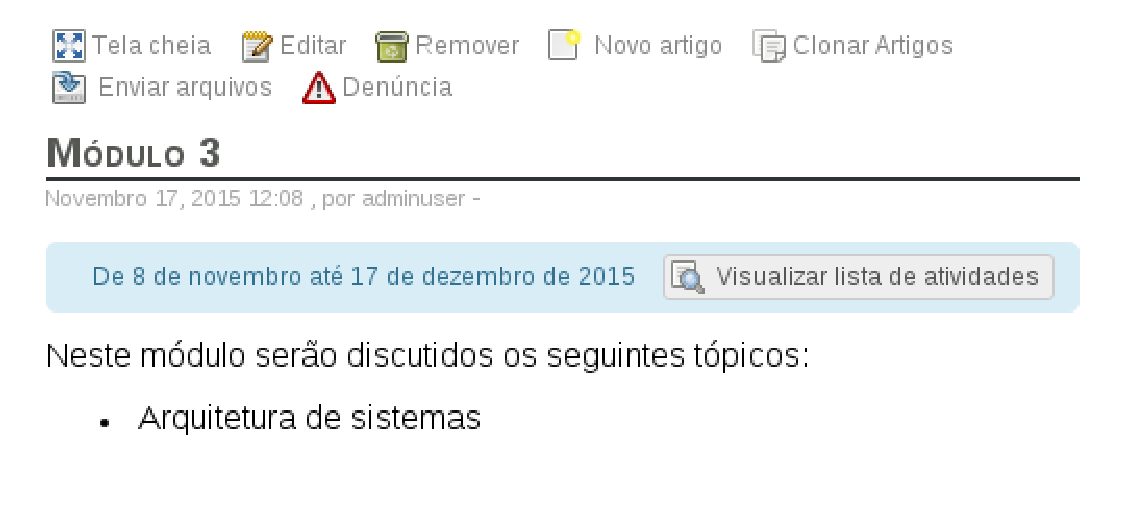
\includegraphics[keepaspectratio=true,scale=0.6]
      {figuras/principal-group.eps}
    \caption{Tela principal de um módulo.}
    \label{fig:principal-group}
\end{figure}

Após salvar esse grupo de trabalho o usuário é redirecionado para o módulo criado. Nesta tela é exibido ao usuário a descrição e o período referentes ao módulo. Existe ainda um botão denominado ``Visualizar lista de atividades'', que mostra ao usuário ou administrador a lista de todas as atividades daquele módulo, conforme mostra a Figura \ref{fig:principal-group}.

\begin{figure}[h]
    \centering
    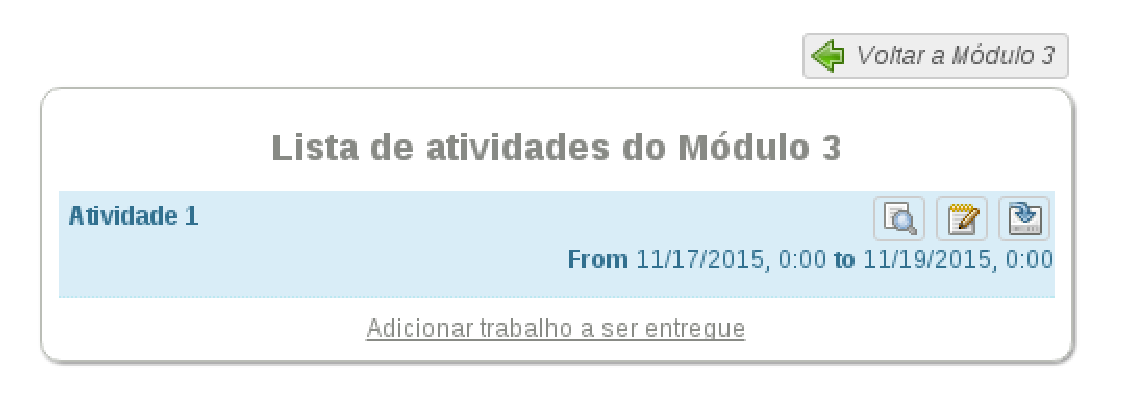
\includegraphics[keepaspectratio=true,scale=0.6]
      {figuras/lista-atividades.eps}
    \caption{Lista de atividades de um \textit{work assignment}.}
    \label{fig:lista-atividades}
\end{figure}

Na Figura \ref{fig:lista-atividades} é exbida a lista de atividades referentes ao módulo criado, com apenas uma atividade, a título exemplificativo. Também é exibido o \textit{link} (``Adicionar trabalho a ser entregue'') que tm a funcionalidade de redirecionar o usuário para a página principal de criação de trabalhos.

\begin{figure}[h]
    \centering
    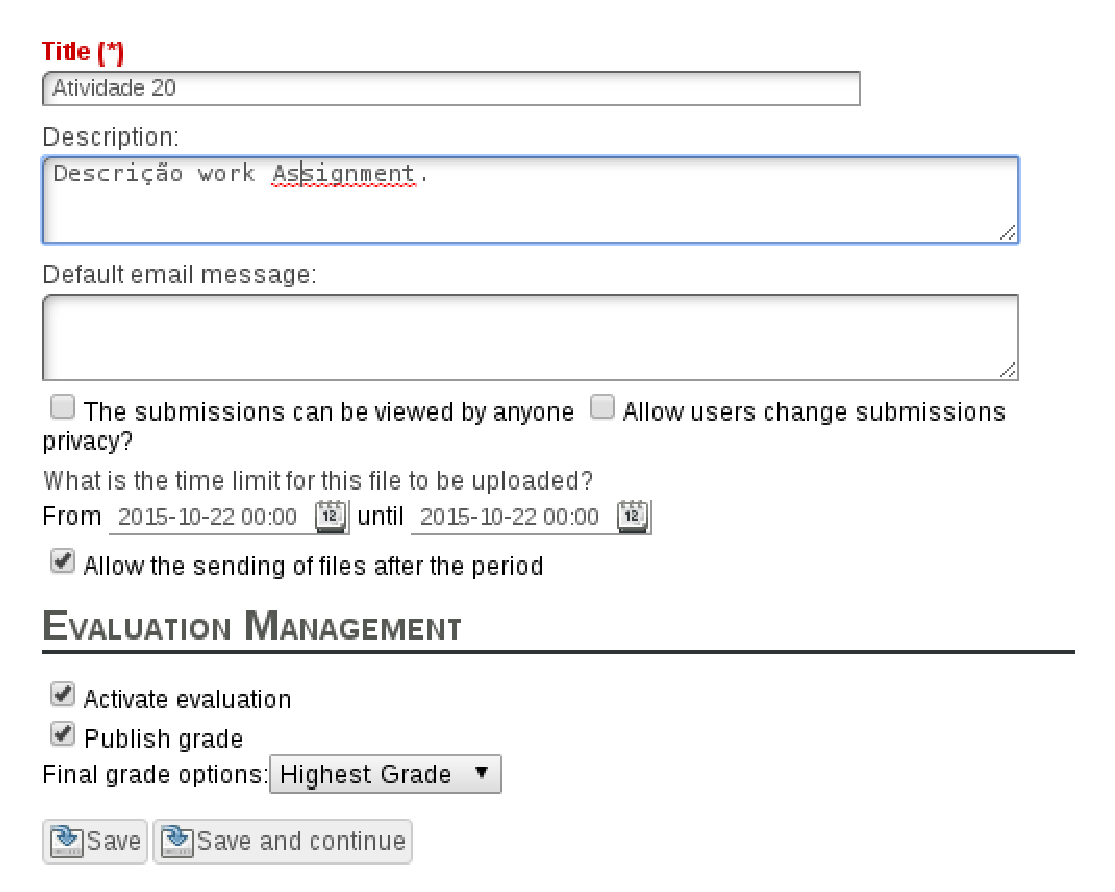
\includegraphics[keepaspectratio=true,scale=0.6]
      {figuras/work-assignment-final.eps}
    \caption{Tela para criação de um \textit{work assignment}.}
    \label{fig:work-assignment-final}
\end{figure}

Nesse conteúdo são solicitadas informações básicas ao usuário sobre o trabalho. Além disso é definido o período que a atividade ficará em aberto e se é possível o envio após a data limite. A Figura \ref{fig:work-assignment-final} também apresenta o gerenciamento das avaliações que permite ativar o modo de avaliação e publicãção de notas de acordo com o critério de avaliação. Como evidenciado na Figura \ref{fig:work-assignment-final} é possível verificar a situação de criação de um novo ``Trabalho a ser entregue''.

\begin{figure}[h]
    \centering
    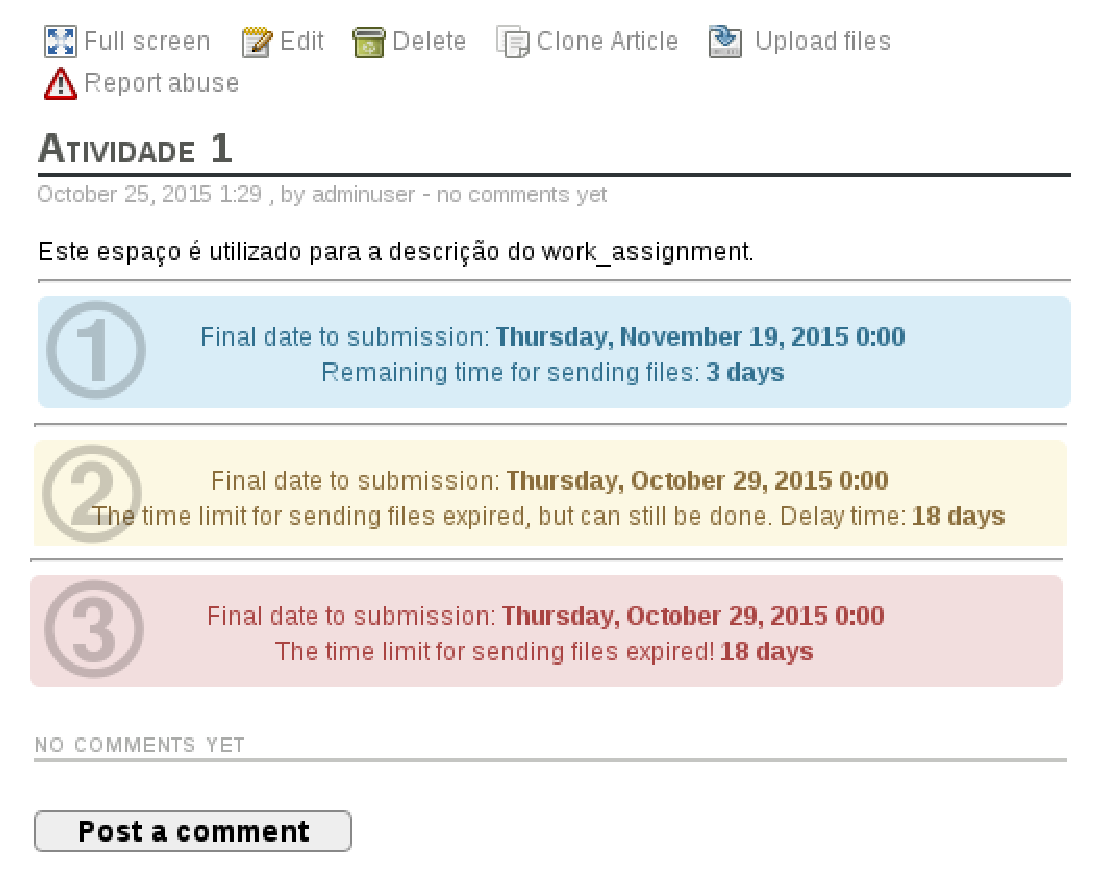
\includegraphics[keepaspectratio=true,scale=0.6]
      {figuras/work-status.eps}
    \caption{Representação do estado dos trabalhos a serem entregues.}
    \label{fig:work-status}
\end{figure}

Como citado, uma das opções deste conteúdo é informar o tempo limite para o envio de arquivos. Buscando a melhor forma de visualização para os usuários foram criados modos de visualização e para isso definiu-se três estados de envio:

\begin{itemize}
\item Aberto: exibe o tempo definido para aquela atividade e o tempo ainda restante para o término do envio (Figura \ref{fig:work-status}, item 1)
\item Permitido: o usuário é informado se o período de envio já expirou e quanto tempo já se passou após a data limite (Figura \ref{fig:work-status}, item 2)
\item Expirado: exibe o tempo definido para a atividade e que a mesma está expirada. (Figura \ref{fig:work-status}, item 3)
\end{itemize}

Para que o usuário visualize a atividade e saiba de imediato em qual situação ela se encontra, foi utilizado um esquema de cores que fica como plano de fundo da notificação que informa o tempo restante. De acordo com a figura \ref{fig:work-status} podemos visualizar que foram utilizadas três cores: o verde para representar que a atividade está em aberto (Item 1), o laranja para informar que é permitido (Item 2), e o vermelho para indicar que está fechada (Item 3). É importante ressaltar que a Figura \ref{fig:work-status} exibe os três estados disponíveis, mas para cada ``Trabalho a ser entregue'' é exibido apenas um de acordo com a situação.

\begin{figure}[h]
    \centering
    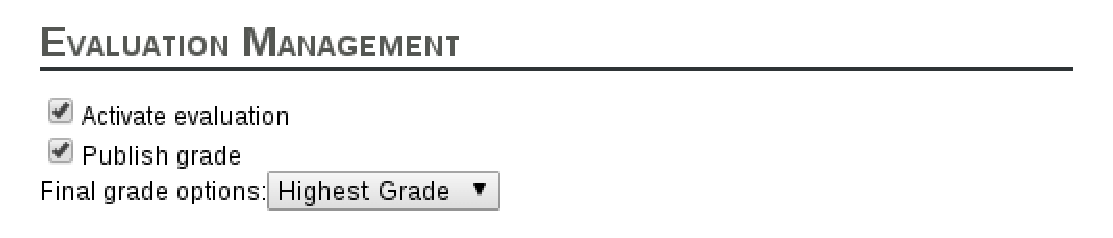
\includegraphics[keepaspectratio=true,scale=0.75]
      {figuras/evaluation-management.eps}
    \caption{Tela para o gerenciamento de avaliações.}
    \label{fig:evaluation-management}
\end{figure}

Ainda na tela para de criação de trabalhos a serem enviados, é importante ressaltar que para cada ``Trabalho a ser enviado'' o administrador pode escolher se deseja ou não publicar as notas para os alunos, permitindo ao mesmo realizar todas as avaliações antes de publicá-las.

O gerenciamento também proporciona ao administrador definir os critérios para a definição da nota final de cada atividade, conforme abaixo:
\begin{itemize}
\item Maior nota: é exibida como nota final a maior nota de todas as versões pontuadas.
\item Mais Recente: é exibida como nota final a última versão pontuada.
\item Nota opcional: no momento da avalição de cada versão o administrador define qual é a nota final
\end{itemize}

Essas funcionalidades proporcionam flexibilidade quanto ao critério de avaliação do professor e fornecem maior liberdade para realizar as avaliações. As opções do gerenciamento de notas estão evidenciadas na Figura \ref{fig:evaluation-management}.

O professor pode pontuar os arquivos enviados pelos usuários, caso tenha habilitado a opção ``Ativar Avaliação''. Como o \textit{plugin} permite o envio de mais de uma versão para a mesma atividade, foi definido que todas elas poderiam ser pontuados. Dessa forma, a nota final é registrada de acordo com os critérios estabelecidos.

\begin{figure}[h]
    \centering
    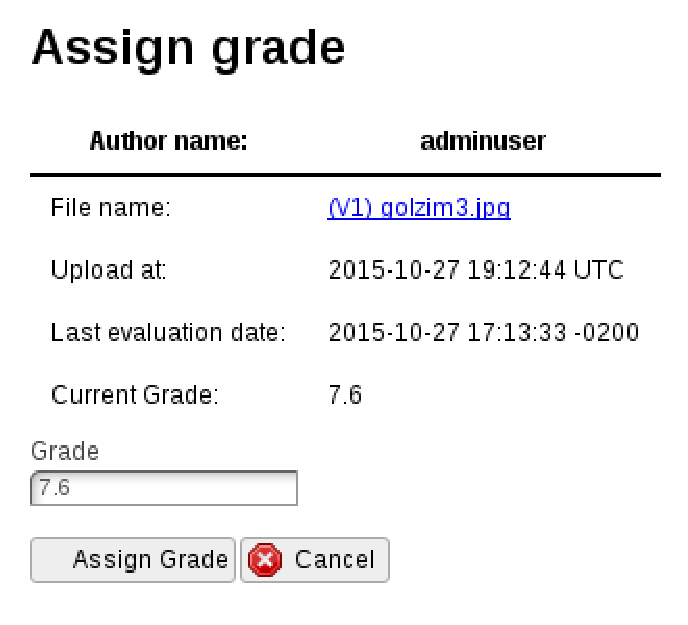
\includegraphics[keepaspectratio=true,scale=0.6]
      {figuras/assign-grade.eps}
    \caption{Tela para atribuição e alteração da notas.}
    \label{fig:assign-grade}
\end{figure}

Na visualização da lista de trabalhos enviados o professor pode selecionar a opção ``atribuir nota'' que o redireciona para a tela que permite atribuir e alterar a nota de cada arquivo enviado, conforme evidenciado na Figura \ref{fig:assign-grade}.

Essa tela (Figura \ref{fig:assign-grade}) exibe ao usuário informações relevantes no momento da avaliação, a exemplo do nome do arquivo a ser avaliado, a data de envio, a data da última avaliação e a nota atual (caso exista) daquele arquivo. Além disso está disponível campo para atribuição de nova nota ao aluno.

\begin{figure}[h]
    \centering
    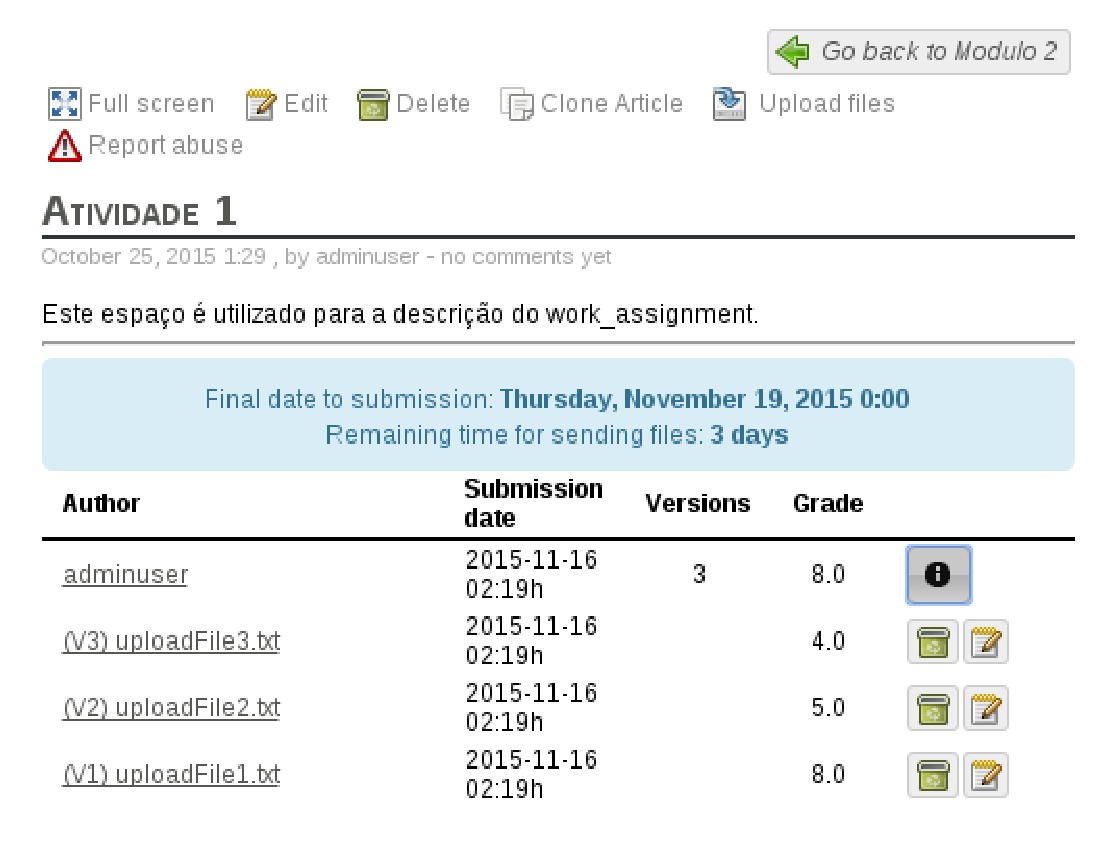
\includegraphics[keepaspectratio=true,scale=0.6]
      {figuras/visualiza-notas.eps}
    \caption{Visualização das notas de trabalhos enviados.}
    \label{fig:visualiza-notas}
\end{figure}

Desde que a avaliação esteja ativa e o administrador tenha permitido a visualização das notas, é criada uma coluna que é exibe a nota final do aluno e a pontuação de cada versão avaliada. Este comportamento é evidenciado na Figura \ref{fig:visualiza-notas}.

Foi implementada uma funcionalidade que tem como principal obejtivo centralizar todas atividades de um usuário e deste modo organizá-las dentro de seus módulos e as comunidades pertencentes.

\begin{figure}[h]
    \centering
    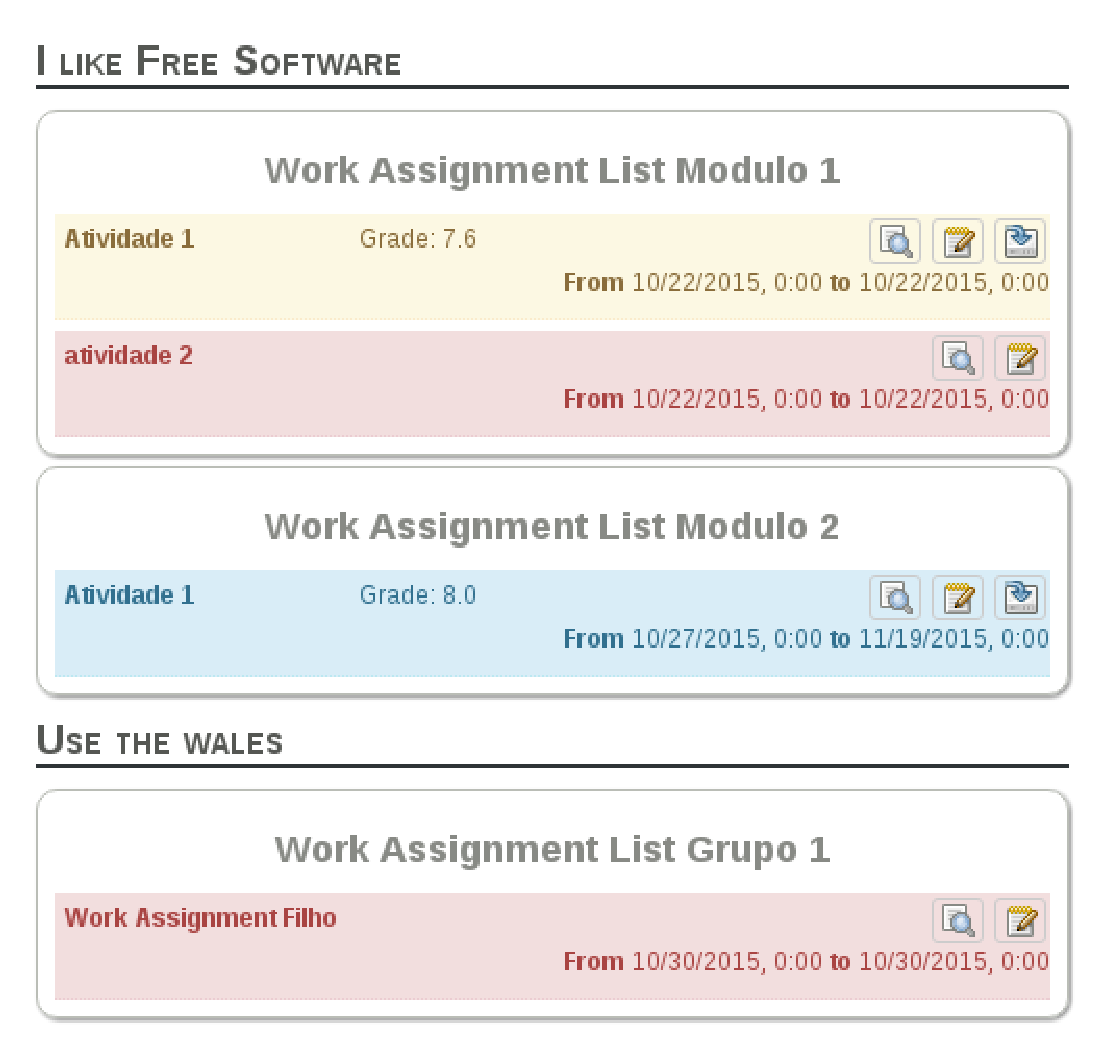
\includegraphics[keepaspectratio=true,scale=0.5]
      {figuras/work-assignment-group-list.eps}
    \caption{Tela para visualização das atividades de forma centralizada.}
    \label{fig:group-list}
\end{figure}

No painel de controle dos usuários, foi criado nova funcionalidade chamada de ``Meus Cursos'' que, ao ser clicada, redireciona o usuário a uma lista de todas as comunidades às quais pertence e que possuem algum tipo de conteúdo relacionado ao grupo de atividades. Conforme evidenciado na Figura \ref{fig:group-list}, são exibidas todas as atividades em seus respectivos grupos.

Utilizando a personalização que o Noosfero oferece, foram criados blocos que fornecem flexibilidade ao usuário quanto ao posicionamento e exibição do mesmo. Esses blocos beneficiam o usuário quanto ao \textit{feedback} sobre suas notas. Conforme pode ser visualizado a esquerda na Figura \ref{fig:blocos}, esse bloco exibe ao usuário as cinco notas mais recentes.

\begin{figure}[h]
    \centering
    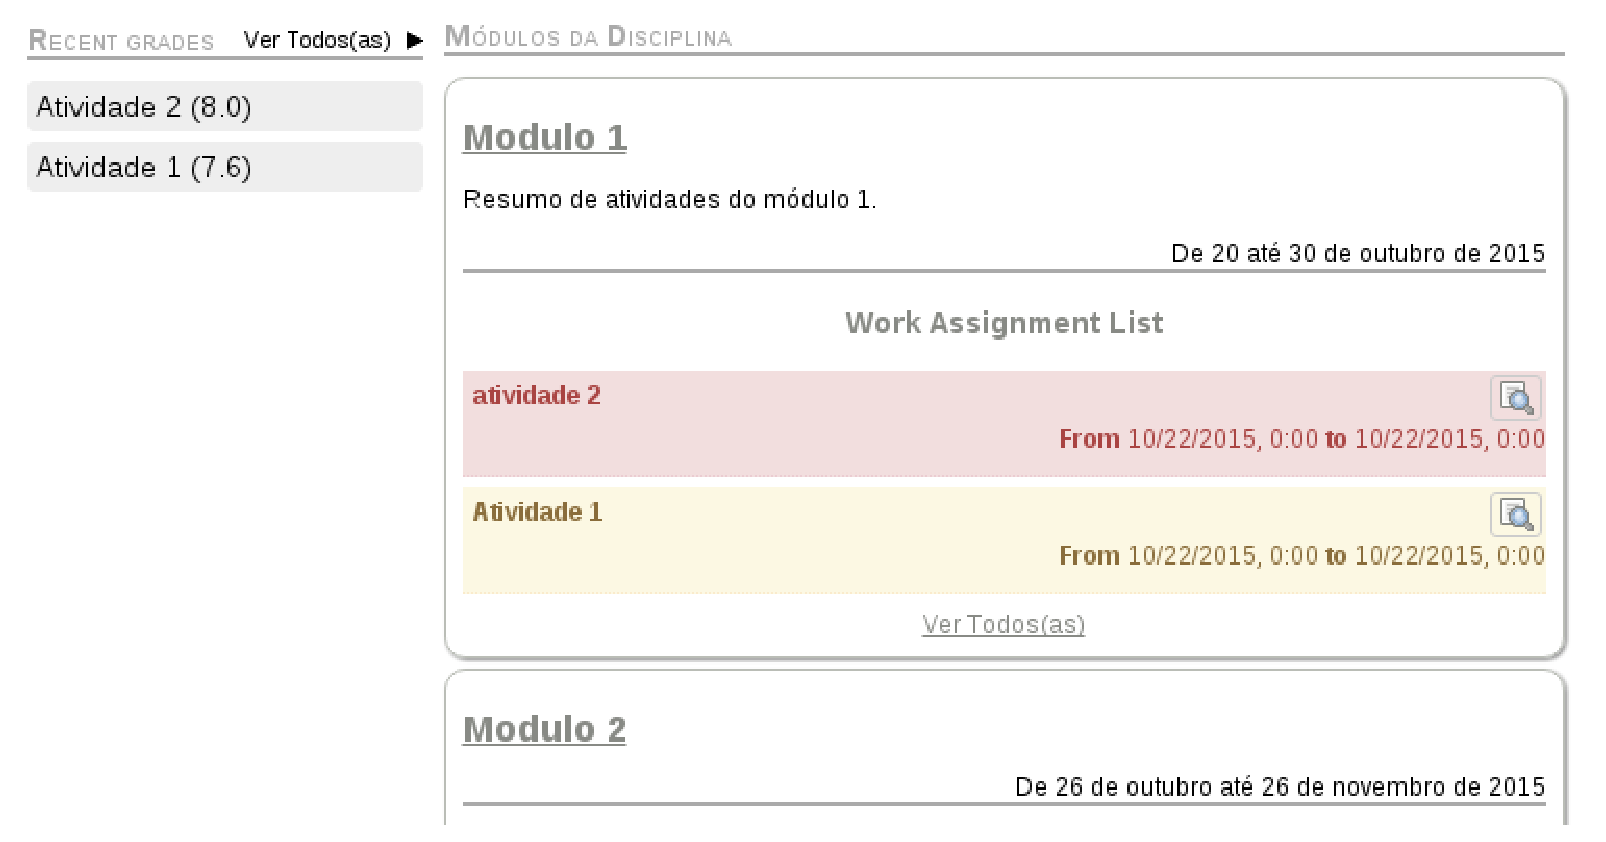
\includegraphics[keepaspectratio=true,scale=0.5]
      {figuras/blocos.eps}
    \caption{Blocos para visualização das atividades.}
    \label{fig:blocos}
\end{figure}


Na Figura \ref{fig:blocos} evidencia-se o bloco para visualização de todos grupos e suas respectivas atividades. Por padrão são exibidas apenas três atividades por grupo, mas é permitido ao administrador da comunidade escolher quantas deseja.

As funcionalidades deenvolvidas são importantes no contexto da UnB, pois, segundo o documento da instituição \citeonline[p. 37]{unb-professor}, as notas para os alunos auxiliam a assimilação progressiva de conhecimento. Sabe-se, ainda que permite maior \textit{feedback} para o aluno, pois nem sempre fica transparente o seu desempenho ao longo do semestre.

Em resumo, as funcionalidades apresentadas neste capítulo colaboram para uso do Comunidade.UnB, tornando-o uma plataforma híbrida entre um ambiente virtual de aprendizagem e uma rede social, para a troca de conhecimento através das comunidades e perfis de usuários. Assim, permite englobar departamentos, organizações e projetos específicos da Universidade.

\subsection{Arquitetura do Plugin Work Assignment}

Sabendo que o Noosfero está em constante evolução o \textit{plugin Work Assignment} passará por melhorias durante sua vida útil. Assim, é importante entender como se onfigura a sua arquitetura após as implementações realizadas, afim de compreender quais classes compõem sua estrutura e como se relacionam.

\begin{figure}[h]
    \centering
    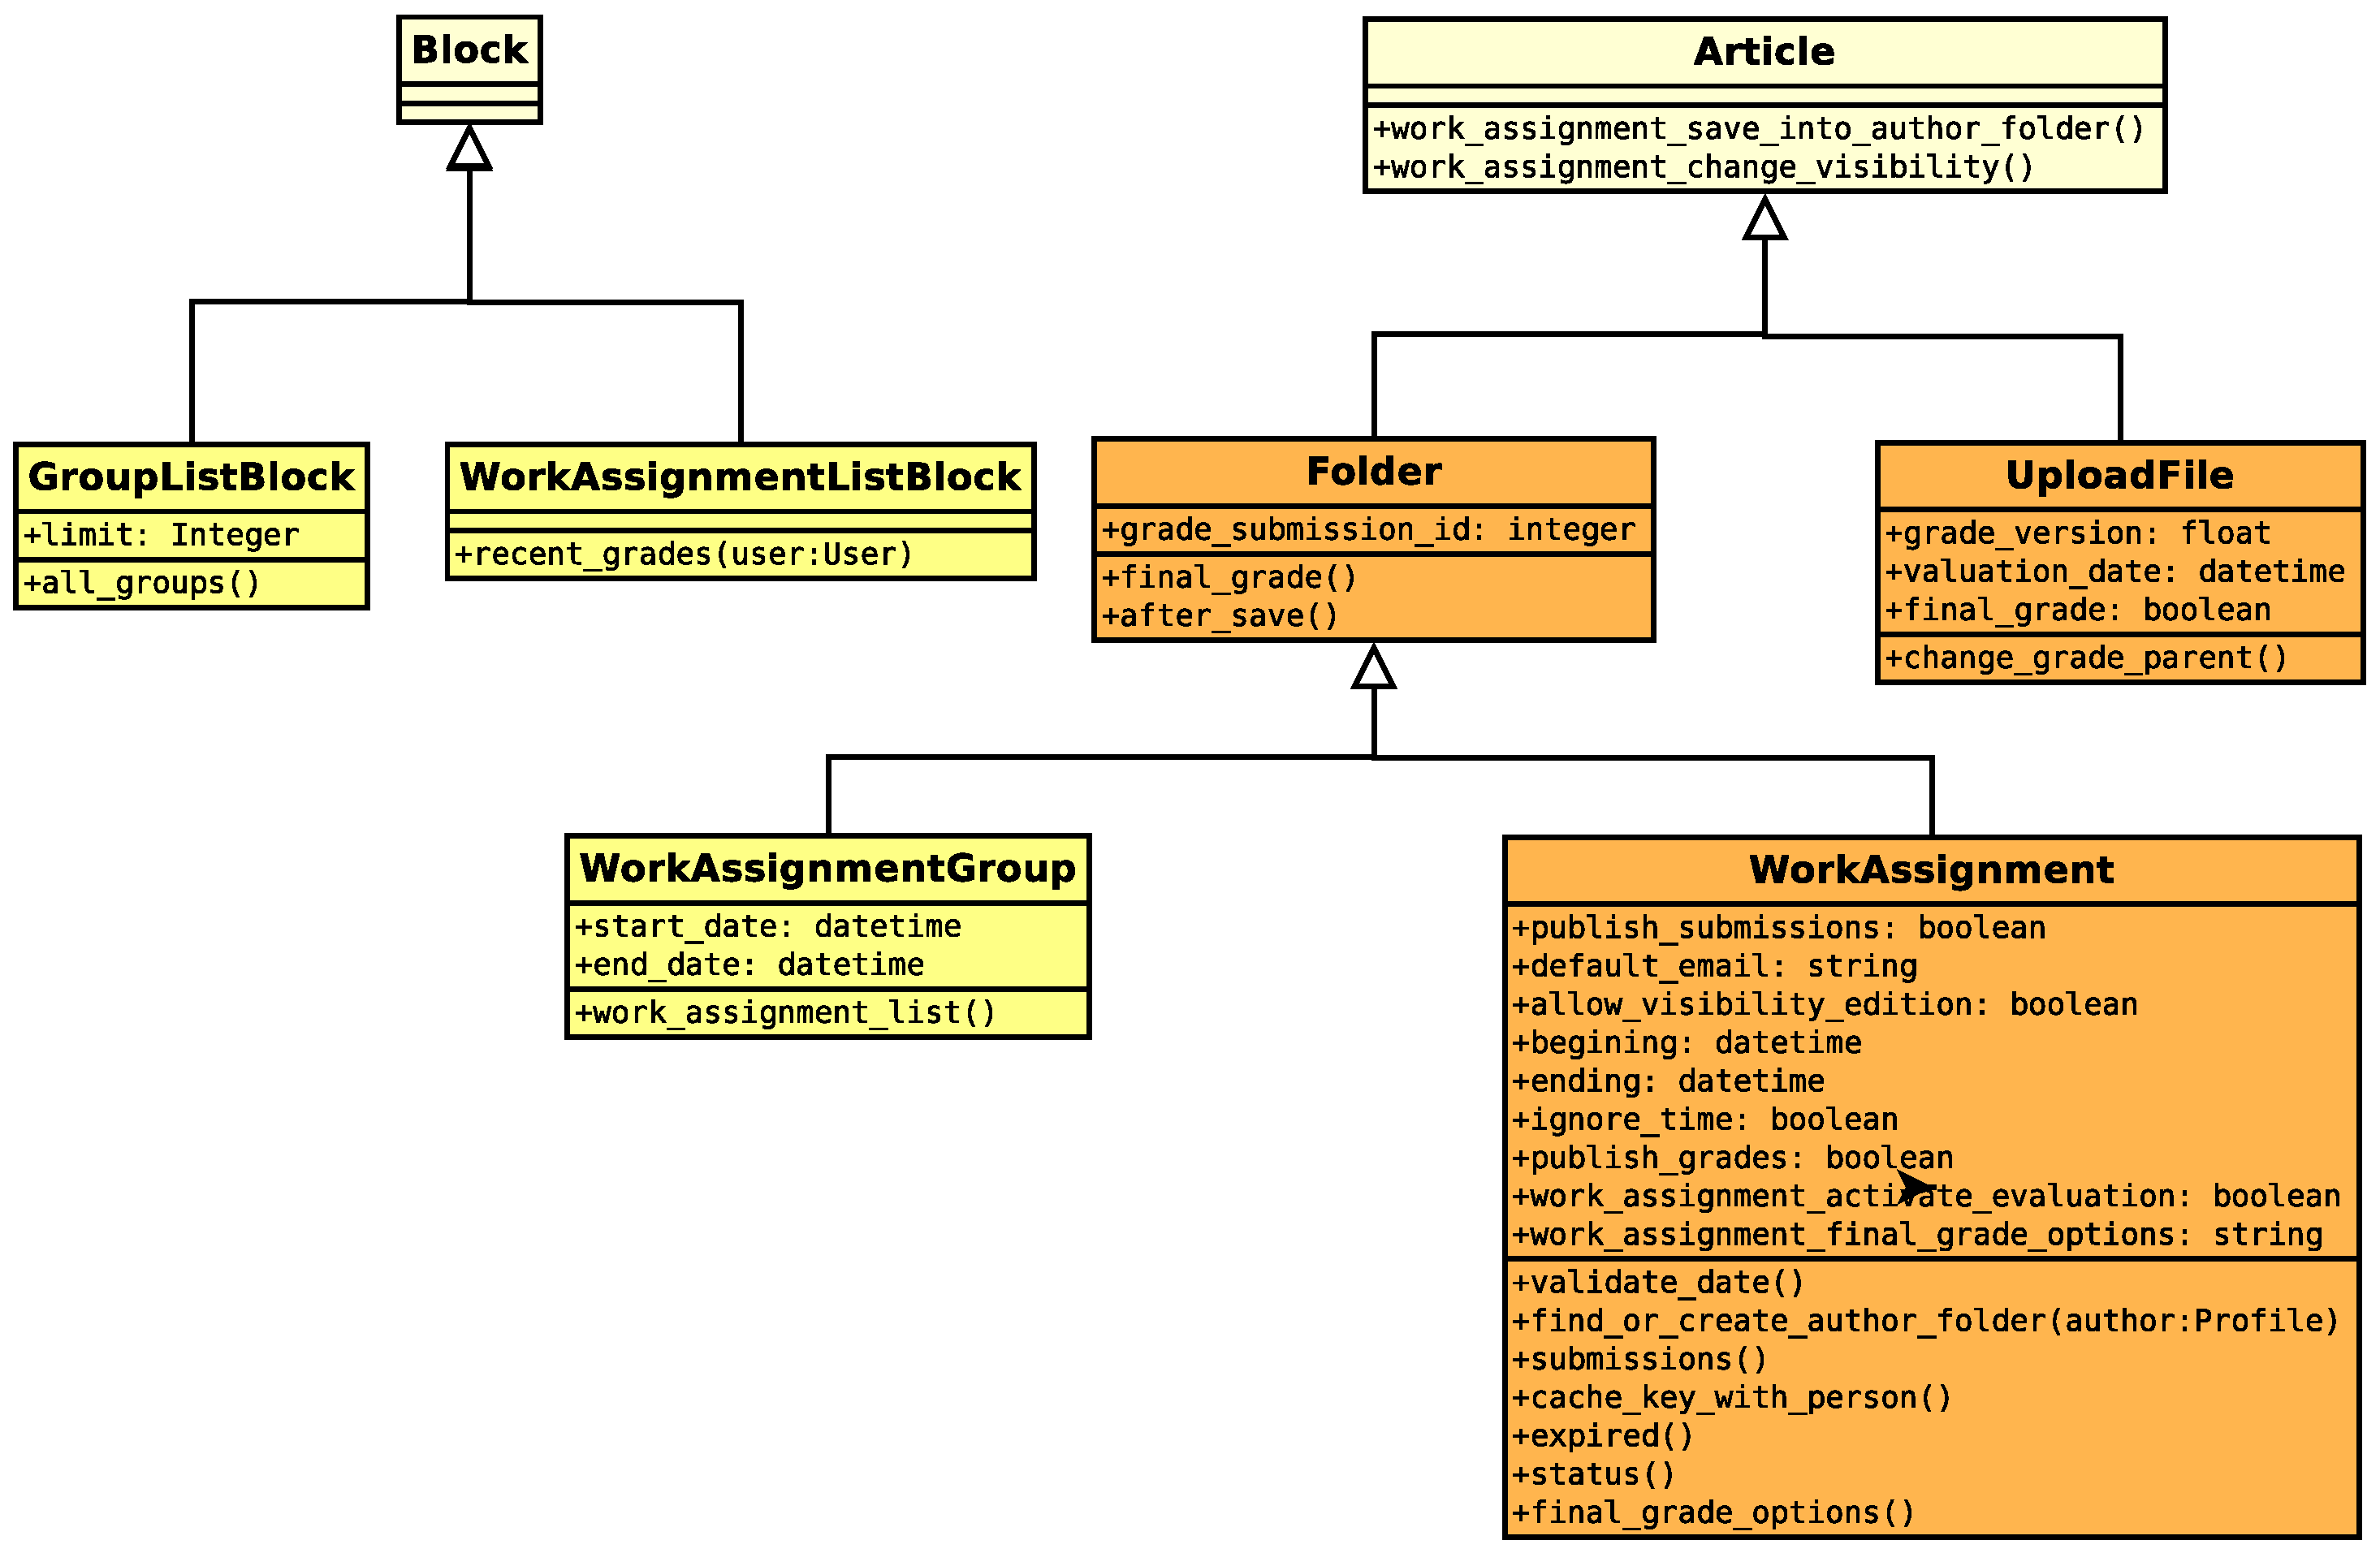
\includegraphics[keepaspectratio=true,scale=0.3]
      {figuras/diagramaUMLCompletoColor.eps}
    \caption{Diagrama de classes do \textit{Plugin Work Assignment}}
    \label{fig:arquitetura-work}
\end{figure}

A Figura \ref{fig:arquitetura-work} evidencia as principais classes utilizadas pelo \textit{plugin}, no qual foram criadas as classes \textit{GroupListBlock, WorkAssignmentListBLock, WorkAssignmentGroup}, e apenas modificadas as \textit{WorkAssignment, UploadFile, Folder} e \textit{Article, Block} que não sofreram modificações durante este processo de evolução.

No desenvolvimento foi criado uma especialização da classe \textit{Folder} denominada como \textit{WorkAssignmentGroup}, que possibilita ao administrador criar pastas que representam grupos de atividades e tem como principal característica a data de início e fim.

No funcionamento do \textit{plugin}, quando um usuário cria um ``Grupo de Atividades'' é possível inserir qualquer tipo de \textit{Article} dentro dessa pasta, possibilitando a criação de um ``Trabalho a ser enviado'' (\textit{WorkAssignment}). A partir disso os membros da comunidade podem enviar seus arquivos como resposta a atividade, e quando o envio é realizado o \textit{plugin} cria uma pasta (\textit{Folder}) para cada usuário e a associa ao arquivo enviado (\textit{UploadFile}). 

Na solução foi considerado o fato de que todos os arquivos enviados por uma única pessoa poderiam ser pontuados, tornando opcional o critério para a nota final. Para isso foram criados dois atributos (grade\_version, valuation\_date) na classe \textit{UploadFile}, que armazenam a nota da versão enviada e a data da avaliação, assim uma vez que a pontuação de uma versão é alterada a nota final do aluno se modifica de acordo com o critério de avaliação.

As classes \textit{WorkAssignmentListBlock} e \textit{GroupListBlock} são uma especialização de \textit{Block} responsáveis por disponibilizar ao usuário a opção de blocos que exibem as notas recentes e listam todos os grupos de uma comunidade, respectivamente.

Entendendo esse funcionamento verifica-se que a arquitetura tornou o \textit{plugin} flexível ao ponto que todas essas classe principais (\textit{WorkAssignmentGroup, WorkAssignment, UploadFile, Folder}) podem ser criadas de forma independente. A dependência está relacionada aos blocos que são dispensáveis caso não existam trabalhos a serem enviados ou grupos de atividades.

\section{A evolução do \textit{plugin Comunidade.UnB}}
\label{plugin-comunidade}

Como o \textit{plugin} permitia que apenas os novos usuários realizassem o cadastro de suas matrículas, foi criada nova versão que permite cadastrar a matrícula dos usuários que já possuem registro no Comunidade.UnB. Dessa maneira, o \textit{plugin Comunidade.UnB} é ativado e permite a autenticação apenas dos usuários cadastrados no LDAP da universidade. Esta base de dados contempla alunos, professores, servidores técnico-administrativos que queiram utilizar a rede. A história de usuário (\ref{us09}) com seus respectivos cenários de uso, encontram-se disponíveis no Seção \ref{historia-usuario}.

\begin{figure}[h]
    \centering
    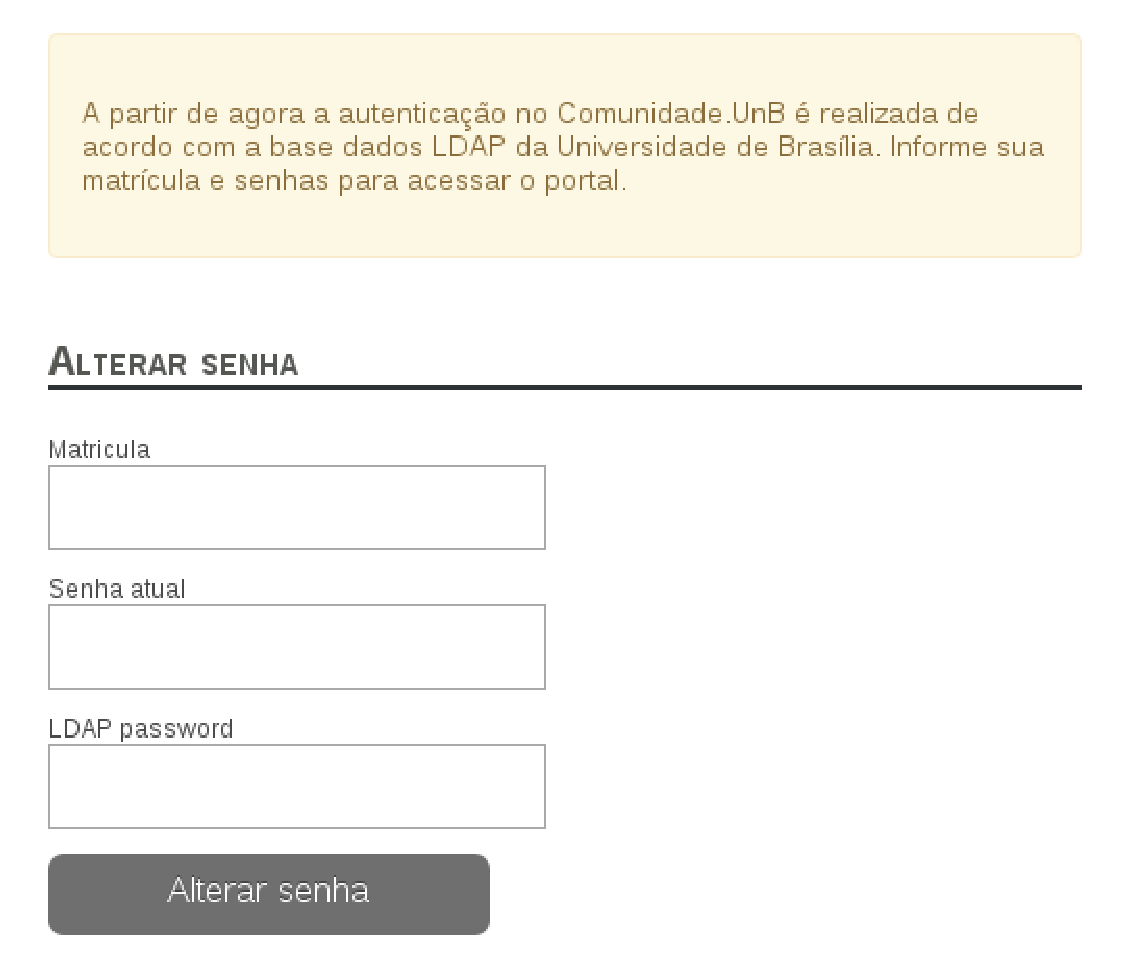
\includegraphics[keepaspectratio=true,scale=0.5]
      {figuras/associate-matricula.eps}
    \caption{Tela para assoicar matricula ao usuário.}
    \label{fig:associate-matricula}
\end{figure}

Com a nova funcionalidade após o usuário realizar o Login, ele é redirecionado para uma tela que solicita a matrícula e senhas do Portal e do LDAP, conforme a Figura \ref{fig:associate-matricula}. O sistema verifica os dados na base de dados LDAP e caso seja confirmado, cadastra matrícula e altera a senha do usuário.

Foi retirada a funcionalidade de alteração e recuperação de senha uma vez que queremos manter a compatibilidade entre a rede Comunidade.UnB e os demais serviços. Desta forma, caso o usuário deseje trocar sua senha, o mesmo deve procurar o CPD e solicitar a alteração.

Com o objetivo de utilizar este \textit{plugin} em um ambiente de produção é necessário solicitar acesso ao LDAP de alunos do matricula web, visto que o da FGA segue um mesmo padrão de senha para todos os usuários, dessa forma todos ficariam com suas contas vulneráveis à acessos indevidos.

Como visto o \textit{plugin} traz para o Comunidade.UnB maior controle sobre seus usuários, centralizando o acesso para o escopo da Universidade.
